\documentclass[10pt,letterpaper]{article}

\usepackage{cogsci}
\usepackage{pslatex}
\usepackage[nodoi]{apacite}
\usepackage{graphicx}
\usepackage[american]{babel}
\usepackage{amsmath}
\usepackage[section]{placeins}
\usepackage{enumitem}
\usepackage{tikz}
\usetikzlibrary{bayesnet}

\title{Linguistic input is coordinated to children's developmental level}
 
 \author{{\large \bf Daniel Yurovsky} \\ \texttt{yurovsky@stanford.edu}\\ Department of Psychology \\ Stanford University
 	\And {\large \bf Gabriel Doyle} \\ \texttt{gdoyle@stanford.edu} \\ Department of Psychology \\ University of California,\\ San Diego
	\And {\large \bf Michael C. Frank} \\ \texttt{mcfrank@stanford.edu} \\ Department of Psychology \\ Stanford University}

\begin{document}

\maketitle

\begin{abstract}

Children rapidly learn a tremendous amount about language despite limitations imposed on them by their developing cognitive processes. One possibility is that caregivers \emph{coordinate} the language they produce to these limitations, titrating the complexity of their speech at developmentally-appropriate levels. We test this proposal by measuring the extent to which parents alter their speech to children in a contingent manner over the course of the first 5 years. Our large-scale corpus analysis confirms this prediction, showing a high degree of mostly parent-led coordination early in development that decreases as children become more proficient language learners and users. 

\textbf{Keywords:} 
Language acquisition, cognitive development, computational models
\end{abstract}

\section{Introduction}

Children learn a tremendous amount about language in their first few years of life. By the time they are able to run down the street, typically developing children have over a thousand words in their productive vocabularies \cite{mayor2011}. They can combine these words to produce new, meaningful multi-word utterances \cite{lieven2009}. They can even use this this budding knowledge to learn new words from just the syntactic constructions in which they occur \cite{yuan2009}.

What explains this rapid acquisition? The last two decades of research have uncovered an abundance of surprising competencies in very young children. By8-months, children can use distributional properties of language to segment discrete words from continuous speech \cite{saffran1996}, and by 12-months can use these same kinds of cues to learn ordering regularities in artificial grammars \cite{gomez1999} and mappings between words and objects \cite{smith2008}. However, while these and other competencies are available early, children's level of \emph{performance} in these domains is often strikingly limited. For instance, children's learning of new words from distributional properties of language is highly constrained by their developing attentional and memory systems \cite{vlach2012, vlach2013}. 

Why do children learn so quickly if their learning is so constrained? One possibility is that child-directed speech differs systematically from speech used to test their learning in the laboratory. Indeed, the language that parents produce to their children---across a variety of levels and structures---appears to contain many redundant cues and regularities that facilitate learning \cite{gogate2000, thiessen2005, yurovsky2012}. However, in some cases child-directed appears systemtically different in ways that do not support learning. For instance, child-directed speech typically contains simpler and less variable syntactic structures. This simplicity is thought to aid in early grammatical acquisition, but also makes it \emph{harder} to learn more complex constructions \cite{montag2015a, montag2015b}. 

The solution, then, may be neither in the learner nor in the input, but in the coordination between learner and input: Parents might fine-tune the complexity of their language to the developing abilities and needs of their budding language learners \cite{snow1972, vygotsky1978}. This fine-tuning hypothesis was initially struck down by two pieces of evidence. First, parents do not appear to use simpler words when speaking to younger children \cite{hayes1988}. Second, parents rarely correct their children's syntactic errors, and children are resistant to the few corrections they get \cite{brown1970, newport1977}. However, a number of more recent studies have shown that parents are more likely to repeat and reformulate ungrammatical utterances, and do so more often for younger children \cite{hirsh-pasek1984, chouinard2003}. Thus, parents may provide subtler, but nonetheless contingent, linguistic cues in a way that is fine-tuned to children's developmental level. 

We pursue this hypothesis in a large-scale corpus study using \emph{linguistic alignment}, a measure of how much speakers change the way they talk to accommodate their conversational partners. Critically, alignment is a local measure---high alignment results not from choosing words that are simpler overall, but from choosing words that easier to process in context \cite<c.f.>{hayes1988}. We predict that caregivers should align more to their younger children, altering their speech more when children need more linguistic support. 

\subsection{Linguistic alignment}

When we use language to communicate, we are trying to use the words we say to convey the message we intend. Some of the words will be obligatory to getting the message across. For illustration, consider the conversation in Table~\ref{tab:naima}. In her first response, Naima's mom has little choice but to say ``sweet potato'' if she wants to inform Naima that they are eating sweet potato. However, she could perfectly well have left out the words ``some,'' ``that,'' and ``this,'' or exchanged them for others and still conveyed the identity of the food on Naima's plate.  

\begin{table}[tb]
\begin{tabular}{r p{.35\textwidth}}
\hline
Naima: & Eating \textbf{that}. Eating \textbf{some of that}.\\

Mom: & \textbf{Some of this}? \textbf{You} know what \textbf{that is}? \textbf{It is} sweet potato.\\

Naima: & \textbf{I} am \textbf{a} bear \textbf{that} eats.\\

Mom: & \textbf{You're a} bear \textbf{that} eats what? What do \textbf{you} eat little bear?\\

Naima: & Fresh pear\\
\hline
\end{tabular}
\caption{\label{tab:naima}A snippet of the transcript between Naima (at 20-mo.) and her mother in the Providence Corpus \cite{demuth2006}. Bolded words are members of the LIWC categories and were included in the model \cite{pennebaker2007}. }
\end{table}

Speakers make these choices for a variety of reasons---from low-level reasons like difficulties of co-articulation to high-level reasons like regional dialects. We focus here one particular reason for these choices: contingency on a conversational partner. In particular, when we talk, we will become more likely to use each-other's expressions, aligning to each other. This kind of alignment appears to be a pervasive property of human social interaction and linguistic communication \cite{giles1991, garrod2004}.  Further, this alignment appears to be useful, facilitating fluent processing of speech, and increasing the probability of successful communication and accomplishment of joint goals \cite{ireland2011, fusaroli2012}. Critically, alignment is directional: even in the same contexts, some speakers will align more than others. For instance, alignment varies across a social hierarchy, with less powerful speakers aligning more to powerful speakers \cite{kacewicz2013}. Thus, linguistic alignment can measure how much a speaker's choice of words reflects an effort to coordinate to a conversational partner. We leverage this property to measure the extent to which parents are altering the way the speak to coordinate with their developing children.

In our analysis, we explicitly focus on the words which are least critical for conveying the content of the message. If Mom shows an increased likelihood of using content words in a way that is contingent on the content words produced by Naima, we can conclude only that they are talking about the same thing. However, if Mom increases her likelihood of using Naima's function words, she must be changing the style of the way she talks in a way that makes it easier for Naima to process. We therefore choose as our target words a set of 676 words falling into 14 categories that Pennebaker and his colleagues have identified in a large body of work as ``strictly non-topical style dimension'' \cite<Linguistic Inquiry and Word Count>{pennebaker2007}. We perform our analyses at the level of categories, to capture both exact repetitions of a conversational partner's words and also reformulations and expansions \cite{chouinard2003}. Thus, in Mom's response, both ``this'' and ``that'' would count as instances of the impersonal pronoun category. These 14 LIWC categories have been used by us and others in previous work examining alignment in a variety of contexts from social media to supreme court proceedings \cite{danescu-niculescu-mizil2012, guo2015}.

\section{Model}
To estimate linguistic alignment between parents and their children, and how it changes over development, we extended the model introduced by \citeA{doyle2016} to measure alignment on social media (Figure~\ref{fig:model}). In this model, a speaker's decision to use or not use a word is driven by two sources: (1) The speaker's baseline probability for using that word category ($\eta^{base}$), and (2) The speaker's change from this baseline due to interacting with the listener ($\eta^{align}$). If the speaker produces a word category more often after it has been used by her conversational partner, we say she has aligned her language. Because the 14 LIWC categories vary widely in their empirical production probabilities (Table~\ref{tab:LIWC}, we formally model alignment as the log-odds increase in a category's use. This measure gives us the ability to detect changes equally well when categories are infrequent (e.g. 1st person singular), and when they are frequent (e.g. indefinite pronouns).

For simplicity, we constrain ourselves only to the effects of the listener's previous utterance on the speaker's response, and thus divide utterances into two categories: those that follow immediately after a category's use, and those that do not. For instance, we code Naima's first response to her mom (that contains an article and an indefinite pronoun) as following an utterance that contains an indefinite pronoun but not an article. We convert all utterances in the corpora into binary vectors with a bit indicating the presence or absence of each of the 14 LIWC categories. We model this bit-vector as a draw from a multinomial distribution with a parameter for each category. For messages not following a category's use, the categories parameter is produced by taking the inverse logit of it's baseline log odds $\left(logit^{-1}\left(\eta^{base}\right)\right)$. If the utterance follows an utterance that contains the category, we say that it's probability of production is the inverse logit of the sum of the baseline and alignment log odds $\left(logit^{-1}\left(\eta^{base} + (\eta^{align}\right)\right)$. This is formally equivalent to estimating an additive effect in a logistic regression model.

\begin{table}[tb]
\centering
\begin{tabular}{|c|c|c|c|} \hline
Category & Examples & Adult & Child\\ \hline
Article & \textit{a, an, the} & .31 & .13 \\
Certainty  & \textit{always, never} & .05 & .01 \\
Conjunction  & \textit{but, and, though} & .22 & .06\\
Discrepancy  & \textit{should, would} & .11 & .04 \\
Exclusive  & \textit{without, exclude} & .12 & ..04\\
Inclusive  & \textit{with, include} & .21 & .07\\
Indefinite pronoun & \textit{with, include} & .45 & .19\\
Negation   & \textit{not, never} & .21 & .11\\
Preposition& \textit{to, in, by, from}  & .38 & .14\\
Quantifier   & \textit{few, many} & .13 & .04\\
Tentative & \textit{maybe, perhaps} & .11 & .03\\
1st person singular  & \textit{I, me, mine} & .05 & .04\\
1st person plural & \textit{we, us, ours} & .09 & .02\\
2nd person pronoun   & \textit{you, yourself} & .33 & .06\\
\hline
\end{tabular}
\caption{Marker categories for linguistic alignment, with examples and probability of appearing in adult and child productions.}\label{tab:LIWC}
\end{table}




Because the LIWC categories vary widely in the production frequencies, we draw the log odds of each from an independent uninformative uniform prior $\left(Uniform\left(-5,5\right)\right)$, which covers more than the range of observed probabilities without putting too probability much mass on extremely large or small values \cite{gelman2008}. Conversely, we put conservative prior on alignment, drawing $\eta^{align} \sim Normal(0,.5)$, regularizing it strongly towards zero. To pool data across participants for robust estimation, we estimate all parameters hierarchically. That is, for instance, we say that there is a population-level of alignment, which generates speaker-levels of alignment, which generate category-levels of alignment. This allows us both to make principled inferences both about how much parents align to their children in general, and about how much specific parents align to their children.

Finally, we let both the probability of using any of these categories ($\beta$), and the probability of aligning ($\alpha$) vary over development. Inspection of posterior parameter estimates showed alignment varied approximately linearly with age, so for simplicity, we formalize $\beta$ and $\alpha$ are linear scalars of ($\eta^{base}$) and ($\eta^{align}$) respectively. 

We can thus test two distinct hypotheses about the way that parents might coordinate to their children's developmental level. If $\beta$ is non-zero, then we can infer that speakers change their baseline likelihood of producing the function words in the 14 LIWC categories over the course of children's development. Thus, if parents' $\beta$ is positive, they are using simpler words earlier in development. Similarly, if $\alpha$ is non-zero, then we can infer that speakers change their level of alignment over development. Thus, if parents' $\alpha$ is negative, they are aligning more to their younger children.


\begin{figure}[tb]
  \begin{center}
    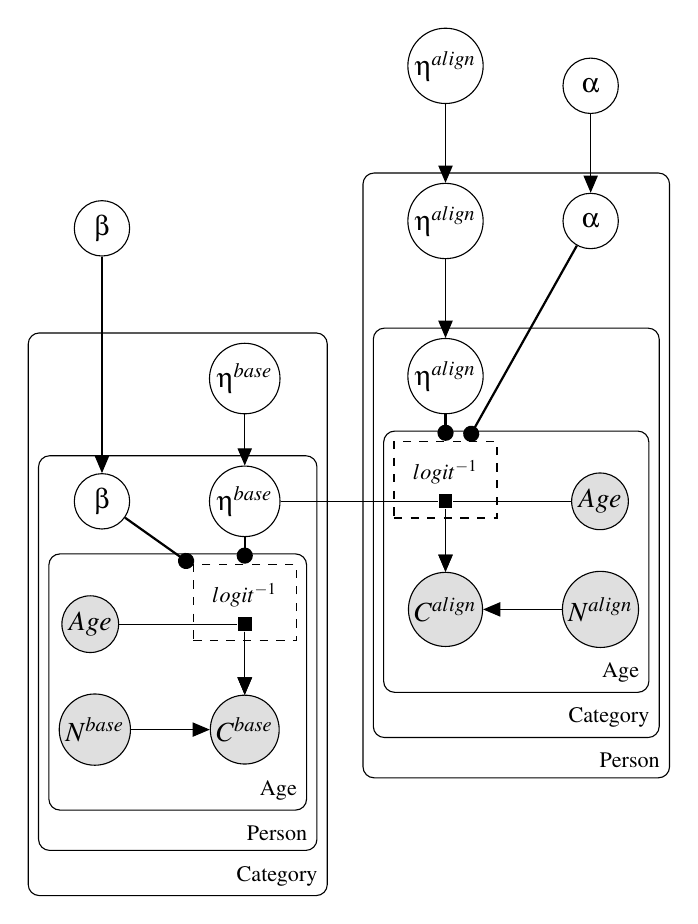
\begin{tikzpicture}[x=1cm,y=1cm]
  
        \node[obs, ]   (C_align)   {$C^{align}$}; %
        \node[obs, right = of C_align]   (N_align) {$N^{align}$}; %
         \node[latent, above = 2 of C_align]   (eta_align_c)   {$\eta^{align}$}; %
         \node[latent, above = of eta_align_c]   (eta_align_p)   {$\eta^{align}$}; %
        \node[latent, above = of eta_align_p]   (eta_align)   {$\eta^{align}$}; %
 	 \factor[above = 0.8 of C_align]       {C_align-f} {$logit^{-1}$} {} {}; %
      
               
          \node[latent, right = of eta_align_p] (age_align_p) {$\alpha$};
          \node[latent, above = of age_align_p] (age_align) {$\alpha$};
      
      
         \gate {logit_align} {(C_align-f)(C_align-f-caption)} {eta_align_c, age_align_p} ; %
         
          \node[obs, right =  1.5 of C_align-f] (Age) {$Age$};

      
       % Nodes
        \node[latent, left = 2 of C_align-f]   (eta_base_p)   {$\eta^{base}$}; %
        \node[obs, below = 2 of eta_base_p]   (C_base)   {$C^{base}$}; %
        \node[latent, above = .65 of eta_base_p]   (eta_base_c)   {$\eta^{base}$}; %
%        \node[latent, above = of eta_base_p]   (eta_base)   {$\eta^{base}$}; %
        \factor[above = 0.8 of C_base]       {C_base-f} {$logit^{-1}$} {} {}; %
        \node[obs, left = of C_base]   (N_base) {$N^{base}$}; %

          \node[obs, left =  1.5 of C_base-f] (Age_base) {$Age$};
      
        \edge{C_base-f}{C_base};
      %  \factoredge {age_align_p} {C_align-f} {C_align} ; 
        \factoredge {Age} {C_align-f} {C_align} ; 
         \factoredge {Age_base} {C_base-f} {C_base} ; 
         
        \node[latent, left = of eta_base_p] (beta_p) {$\beta$};
        \node[latent, above = 2.75 of beta_p] (beta) {$\beta$};

        \edge{eta_base_c}{eta_base_p};
        \edge{age_align}{age_align_p};
  %      \edge{eta_base}{eta_base_p};
        
        \edge{eta_align_p}{eta_align_c};
        \edge{eta_align}{eta_align_p};
        
         \edge{beta}{beta_p};

        \edge {N_base} {C_base};
        \edge {N_align} {C_align};
	 \edge{C_base-f}{C_base};
	 
        \gate {logit_base} {(C_base-f)(C_base-f-caption)} {eta_base_p,beta_p} ; %

        
        \factoredge {eta_base_p} {C_align-f} {C_align} ; %

	\plate {plate_a} {(C_align)(C_align-f)(N_align)(logit_align)(Age)} {Age}; %
	\plate {plate_c} {(C_align)(eta_align_c)(C_align-f)(N_align)(logit_align)(Age)(plate_a)} {Category}; %



	\plate {} {(eta_align_c)(C_align-f)(logit_align)(eta_align_p)(plate_c)(C_align)(N_align)(age_align_p) (Age)(plate_a)}{Person}; %

	
	\plate {plate_a_base} {(C_base)(C_base-f)(N_base)(logit_base)} {Age}; %
	\plate {plate_p_base} {(beta_p)(C_base)(eta_base_p)(C_base-f)(N_base)(logit_base)(plate_a_base)} {Person}; %
	\plate {} {(eta_base_c)(C_base-f)(logit_base)(eta_base_p)(plate_p_base)(C_base)(N_base)(plate_a_base)(eta_base_p)} {Category}; 

\end{tikzpicture}
  \end{center}
  \caption{The Hierarchical Alignment Model (HAM) used to analyze linguistic alignment in CHILDES. Speaker's word choices are modeled as having two influences: (1) Their baseline probability of using each word category ($\eta_{base}$), and (2) Their increase from baseline due to their conversational partner's use of each category in the previous utterance ($\eta_{align}$).}
  \label{fig:model}
\end{figure}

\section{Experiments}

\subsection{Data}

To maximize the power and generalizability of our analysis, we selected all of the English-language transcripts available in CHILDES that contained conversations between a parent and a target child who was 12--60-mos. of age \cite{macwhinney2000}. This resulted in a total of 3,851 transcripts across 417 unique children. The number of transcripts per child varied widely, ranging from 1 ($n = 164$) to 440 ($n = 1$), with a median of 26. 

For each transcript, we first combined all successive utterances from the same speaker into one utterance. We then transformed each utterance into a binary vector with a value for each of the 14 LIWC categories \cite{pennebaker2007}. We then formatted the utterances as a series of message-reply pairs, in which each utterance was treated as a reply to the previous utterance, and a message for the next utterance.

\subsection{Analysis}

For each pair of speakers $A$ and $B$  in a transcript, we then computed four counts for each of the 14 LIWC categories: The number messages from $A$ to $B$ contained the category ($N^{align}$), the number of messages from $A$ to $B$ not containing the category ($N^{base}$), the number of replies containing the category to messages containing the category ($C^{align}$), and the number of replies containing the category to messages not containing the category ($C^{base}$). To generate robust parameter estimates, aggregated counts across all transcripts for the same parent and child into 6-mo. age bins, yielding 8 bins (youngest: 12--18 mo., oldest 54--60 mo.) When estimating $\alpha$ and $\beta$---the age-related scalars in the model, we numbered these bins from 1 to 8 and then subtracted the mean bin number from each (4.5). This centers the intercept ($\eta^{align}$) at the middle value, yielding the smallest average predictive error for other age bins. 

The Hierarchical Alignment Model was then fit to the data separately for children and adults. Posterior distributions for all parameters were estimated using a Hamiltonian Monte Carlo sampler with three independent chains, and 500 samples in each chain. The first 100 samples of each chain were discarded to ensure sufficient burnin based on inspection of trace plots that typically showed convergence after 50-75 samples. In addition, to provide a baseline for comparison, alignment was also estimated for the parent-parent interactions in the corpus. Because these were quite sparse relative to parent-child interactions, and because we had no apriori reason to expect that parents would align differently to each-other over their children's development, they were not separated into distinct age bins.

\subsection{Results and Discussion}

The transcripts in CHILDES span a wide range of typical childhood activities---book reading, toy play, dinner, etc. In all of these activities, however, parents and their children use language for common purpose: to communicate. Because successful communication is facilitated by linguistic alignment,  we predict that both parents and their children show reliably positive levels of alignment. Our model confirms this prediction, producing posterior parameter estimates that are above-zero for both parents and children (Figure~\ref{fig:model_parameters}). We also see that parents align reliably more to their children than their children align to them, and that parents also align reliably more to their children than to each-other. Thus, in the aggregate, we can conclude that parents coordinate to their children more than they coordinate to other adults. This is in line with other work showing that child-directed speech is different from adult-directed speech.

The fine-tuning hypothesis predicts, however, that parents should change the way they talk to their children in a way that is sensitive to their developmental level. One way they could accomplish this would be to change the words they producing, using simpler words with younger children. If so, we would expect an increase in their likelihood of producing optional function words (positive $\beta$). In line with previous analyses, we find no evidence of this \cite{newport1977, hayes1988}. We do, however, find a large and reliable increase in children's use of these words as they grow older, as would be expected from their syntactic development.

Alternatively, parents could use the same words, but be less contingent on children's production---repeating less, clarifying less, rephrasing less. This is precise what we observe---parental alignment decreases reliably over development, and children's alignment shows a similar trend. Thus, parent-child conversations become gradually less coordinated over development, as children need less scaffolding to be successful communicators (Figure~\ref{fig:all_hpds}).

\begin{figure}[tb]
 \center{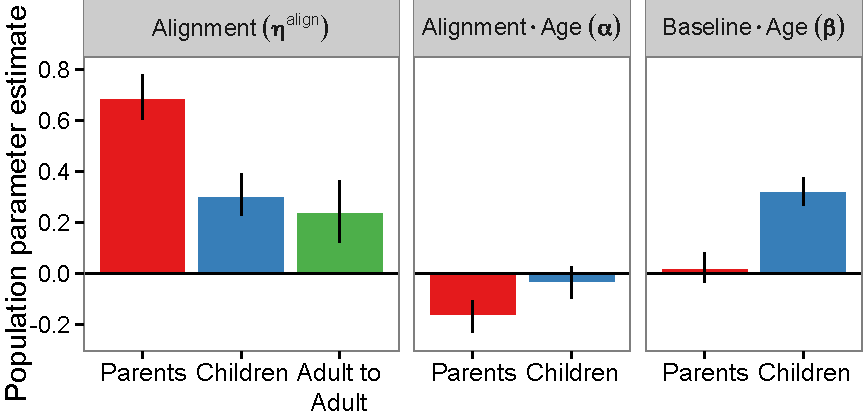
\includegraphics[width=.45\textwidth]{figures/model_params.pdf}}
  \caption{\label{fig:model_parameters} Posterior parameter estimates for population levels of alignment ($\eta^{align}$), fine tuning ($\alpha$), and coarse tuning ($\beta$) both parents and children, as well estimated parent-parent alignment for a baseline. Bars indicate means, and error-bars indicate the 95\% highest posterior density intervals.}
\end{figure}

\begin{figure*}[t]
	\center{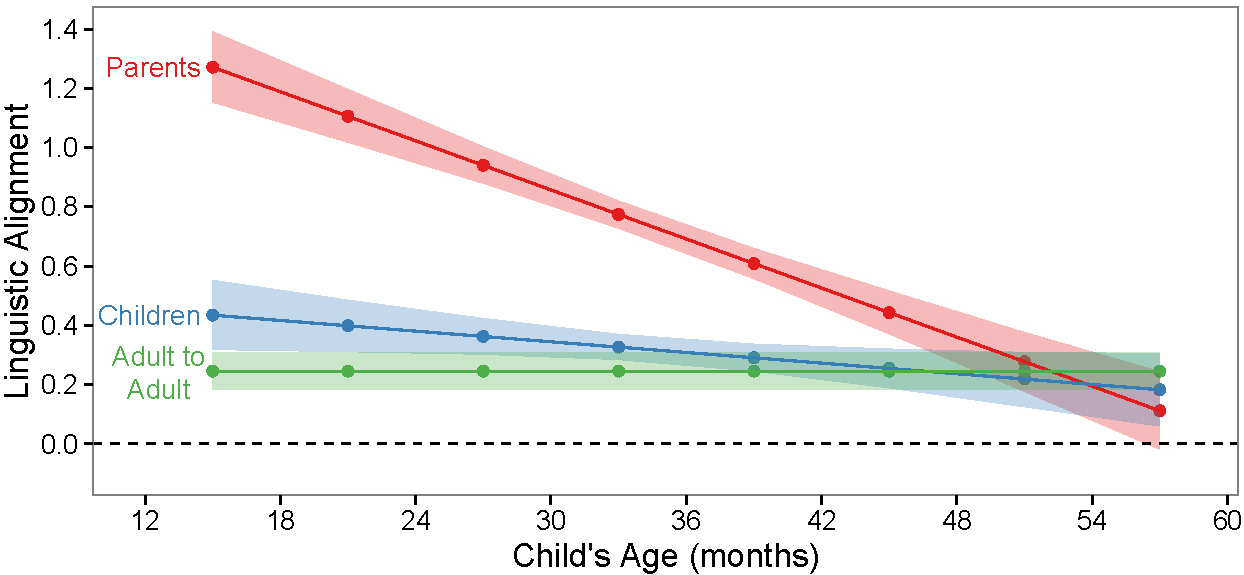
\includegraphics[width=.95\textwidth]{figures/all_hpds.pdf}}
	\caption{Model-estimated changes in linguistics alignment by 6-month-window. Over the course of development, both parents and children decrease in their linguistic alignment until they are indistinguishable from adult-adult interaction baselines. Points indicate the mean of the posterior distribution, lines and shaded regions indicate 68\% highest probability density intervals, equivalent to one standard deviation. 
\label{fig:all_hpds} }
\end{figure*}

In addition to estimating population-level parameters for alignment and fine-tuning, our hierarchical model also estimates parameters for each of the individual adults and children in CHILDES. Examining these parameters shows both the consistent patterns, and the range of variability across parents and children. Figure~\ref{fig:providence_hpds} shows estimated alignment over development for each of the 6 children measured longitudinally in the Providence corpus \cite{demuth2006}. We see consistently across children that parental alignment is highest early in development. However, both children and parents vary in both their level of alignment and in the rate at which it changes across development. Although the nature of the data in CHILDES does not allow us to discover either the sources of the consequences of the individual differences, they suggest a promising a promising future direction for understanding the incredible variation in children's language acquisition.

\begin{figure}[tb]
 \center{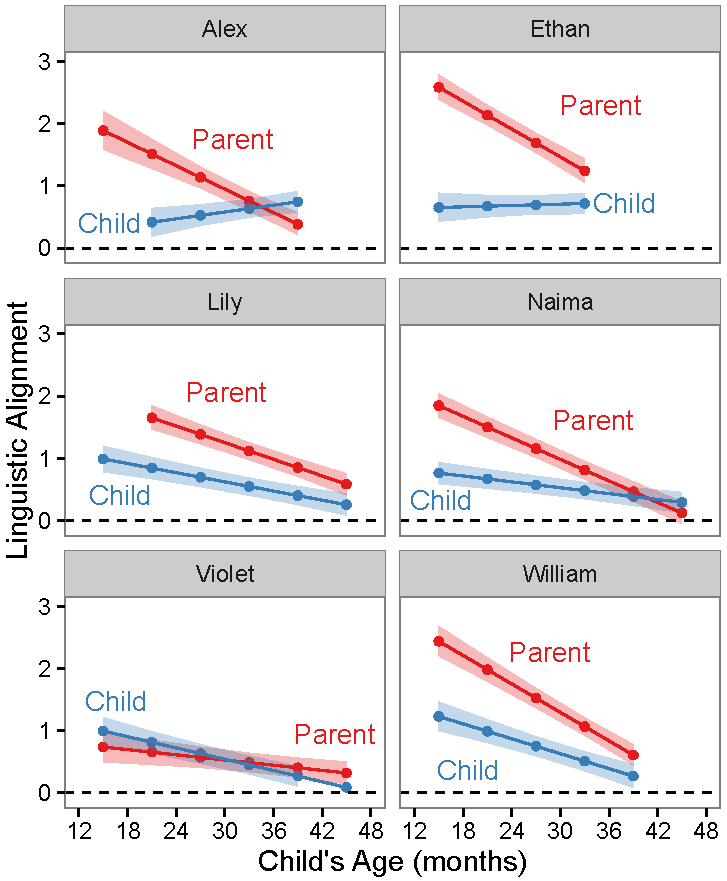
\includegraphics[width=.48\textwidth]{figures/providence_hpds.pdf}}
  \caption{\label{fig:providence_hpds} Model parameters.}
\end{figure}

Repetition vs. Category stuff here?

\section{General Discussion}

%
% For instance, prosodic properties of child-directed speech are believed to be beneficial for learning phonological acquisition \cite{fernald1989, kuhl1997}. However, recent work suggests that some of the properties may make learning adult-like vowels \emph{hard} \cite{mcmurray2013}. 

%puzzles is to consider that these learning processes all unfold over development: The learning problem faced by 6-month-olds is different from the learning problem faced by 2-year-olds, and similarly the learning capacities of a 6-month-old are different from those of a 2-year-old. We propose that the explanation for rapid language acquisition lies neither in the child's early competence, nor in the structure of the input alone; language learning emerges from the  \emph{coordination} between children's developing competencies and the input their caregivers provide \cite{vygotsky1978}. 
%
%If this hypothesis is correct, child-directed speech should be neither uniformly helpful nor uniformly harmful---child directed speech itself should not be uniform. Instead, the structure of linguistic input should be non-stationary, changing as children develop, learn, and become more competent speakers themselves \cite{elman1993, fausey2016}. This is because child-directed speech is not an independent property of the world---it as an action taken by caregivers to communicate with their children. To communicate successfully, caregivers must be mindful of the cognitive and linguistic capacities of their children, and tailor their speech accordingly. 

But changes in competencies suggest that different things need to be scaffolded at different times. Proposal: all input is not created equal, easier input earlier \cite{elman1993, fausey2016}.

Previous work \cite{sokolov1993,dale2006}

desirable difficulties, goldolicks

Local vs global \cite{onnis2008, goldstein2010}

Broader communicative framing, what it means to study distributional learning in a communicative context



\section{Acknowledgments}

We are grateful to Aaron Chuey and Jake Prasad for help with an earlier version of the model. This work was supported by NIH NRSA F32HD075577 to DY and STUFF FOR GABE AND MIKE.

\bibliographystyle{myapacite}

\setlength{\bibleftmargin}{.125in}
\setlength{\bibindent}{-\bibleftmargin}

\bibliography{alignment}


\end{document}
